\documentclass[11pt,a4paper]{article}
\usepackage[T1]{fontenc}
\usepackage[utf8]{inputenc}
\usepackage[french]{babel}
\usepackage{lmodern}
\usepackage{geometry}
\geometry{margin=2.5cm}
\usepackage{amsmath,amssymb,booktabs,array}
\usepackage{graphicx}
\usepackage{float}
\usepackage{xcolor}
\usepackage{fancyhdr}
\usepackage{hyperref}
\hypersetup{colorlinks=true,linkcolor=blue!55!black,urlcolor=blue!55!black,citecolor=blue!55!black}
\pagestyle{fancy}
\fancyhf{}
\fancyhead[L]{Projet 37 -- Commerce agricole Maroc--Afrique}
\fancyhead[R]{Data Science et commerce international}
\fancyfoot[C]{\thepage}
\setlength{\headheight}{14pt}
\begin{document}
\begin{titlepage}
\centering
{\Large ENCG Casablanca \par}
\vspace{1cm}
{\large Filière : Commerce International \quad Module : Data Science\par}
\vspace{1.8cm}
{\huge\bfseries Commerce agricole Maroc--Afrique : analyse en panel et prévision des exportations marocaines de légumes et de fruits (HS07 et HS08)\par}
\vspace{1.5cm}
{\Large Rapport scientifique de projet -- Projet 37\par}
\vspace{1.5cm}
\begin{tabular}{rl}
Étudiant(e) 1 : & Nom Prénom 1 \\
Étudiant(e) 2 : & Nom Prénom 2 \\
Responsable : & A. Larhlimi \\
Année universitaire : & 2026--2027 \\
Date de remise : & JJ/MM/AAAA \\
\end{tabular}
\vfill
\textit{Tous les chiffres, tableaux et figures de ce rapport sont produits par le notebook du projet à partir des données UN Comtrade extraites le 19/11/2026. Aucune valeur n'a été simulée.}
\end{titlepage}

\section*{Résumé}\addcontentsline{toc}{section}{Résumé}
Ce rapport étudie les exportations marocaines de légumes (chapitre HS07) et de fruits (chapitre HS08) vers quinze marchés africains entre 2010 et 2024. Les données proviennent de l'API publique UN Comtrade (\url{https://comtradeapi.un.org/public/v1/preview/C/A/HS}) : 346 lignes brutes, ramenées après nettoyage à un panel de 450 observations pays--chapitre--année. La question est double : quels marchés achètent le plus et progressent le plus, et l'historique permet-il de prévoir la valeur de l'année suivante ? Cinq figures décrivent la structure des flux, puis trois approches de prévision sont comparées avec une validation strictement chronologique : la persistance (référence), une régression Ridge et une forêt aléatoire. Les trois premiers marchés (Mauritanie, Sénégal et Mali) concentrent 79,8~\% de la valeur cumulée. Sur les années cibles 2023--2024, l'erreur absolue moyenne est de 0,809 million(s) USD pour la persistance, 1,165 pour Ridge et 0,896 pour la forêt aléatoire. Aucun modèle appris ne fait mieux que la persistance ; le plus proche, Ridge, a une erreur supérieure de 43,9 \%. Les principales limites sont la brièveté des séries annuelles, l'expression des valeurs en dollars courants, la fréquence des zéros commerciaux (23,1~\% du panel) et l'absence de variables explicatives externes, qui interdit toute lecture causale.

\setcounter{tocdepth}{1}
\tableofcontents
\newpage

\section{Introduction}\label{sec:intro}
\subsection{Contexte économique}
L'agriculture est l'un des premiers secteurs exportateurs du Maroc. Les stratégies publiques successives, le Plan Maroc Vert (2008--2020) puis Génération Green (2020--2030), ont fait du développement des exportations de fruits et légumes un objectif explicite~\cite{agri}. L'Union européenne reste le premier débouché de ces produits ; cette dépendance expose toutefois les exportateurs aux changements de réglementation et de demande sur un seul ensemble de clients. La diversification vers le continent africain est donc régulièrement présentée comme un relais de croissance, dans un contexte marqué par le retour du Maroc au sein de l'Union africaine en 2017 et par le démarrage des échanges dans le cadre de la Zone de libre-échange continentale africaine (ZLECAf) en janvier 2021~\cite{zlecaf}.

Les produits concernés sont périssables. Leur exportation vers l'Afrique subsaharienne dépend de la chaîne du froid, des délais de passage aux frontières et du coût du transport routier, qui emprunte principalement l'axe reliant le Maroc à la Mauritanie puis à l'Afrique de l'Ouest. On s'attend donc à des flux inégaux selon les destinations et sensibles aux campagnes agricoles. Avant d'engager des moyens de prospection, un exportateur ou un organisme de promotion a besoin de deux informations : où se trouvent aujourd'hui les montants, et ce que l'on peut raisonnablement anticiper pour l'année suivante.

\subsection{Problématique et hypothèses}
La question de recherche est la suivante : \emph{quels marchés africains importent davantage de fruits et légumes marocains, et l'historique des flux permet-il de prévoir leur évolution d'une année sur l'autre ?} Trois hypothèses sont testées.
\begin{itemize}
\item \textbf{H1 -- Concentration.} Les flux sont concentrés sur un petit nombre de partenaires proches, principalement en Afrique de l'Ouest.
\item \textbf{H2 -- Persistance.} Les relations commerciales sont inertes : la valeur de l'année $t$ est le principal prédicteur de la valeur de l'année $t+1$.
\item \textbf{H3 -- Non-linéarité.} Un modèle non linéaire (forêt aléatoire) prévoit mieux qu'un modèle linéaire régularisé (Ridge).
\end{itemize}

\subsection{Objectifs}
\begin{enumerate}
\item Construire un panel traçable des exportations marocaines HS07 et HS08 vers quinze partenaires africains sur 2010--2024, avec un journal des transformations.
\item Décrire la structure des flux (évolution, concentration, croissance, spécialisation, régularité) au moyen de cinq figures interprétées.
\item Comparer une méthode de référence et deux modèles de prévision à un an, sans fuite temporelle, puis mesurer la sensibilité des conclusions.
\end{enumerate}

\section{Présentation du jeu de données}\label{sec:data}
\subsection{Source, période et unité d'analyse}
Les données proviennent de UN Comtrade, la base de statistiques du commerce international de marchandises tenue par la Division de statistique des Nations Unies~\cite{comtrade}. Elles sont extraites par le point d'accès public \emph{preview} \url{https://comtradeapi.un.org/public/v1/preview/C/A/HS} (marchandises, fréquence annuelle, nomenclature du Système harmonisé), avec les paramètres suivants : déclarant Maroc (\texttt{reporterCode=504}), flux d'exportation (\texttt{flowCode=X}), chapitres \texttt{cmdCode=07} et \texttt{08}, quinze partenaires africains (Mauritanie, Sénégal, Côte d'Ivoire, Mali, Burkina Faso, Guinée, Gabon, Cameroun, Tunisie, Algérie, Égypte, Nigeria, Ghana, Kenya, Afrique du Sud) et années 2010 à 2024.

Ce point d'accès ne demande pas de clé mais renvoie au plus 500 lignes par requête et limite la fréquence des appels. L'extraction est donc découpée par chapitre et par groupe de cinq années, avec une pause entre deux appels et un repli année par année lorsqu'une réponse est vide ou plafonnée. Origine des données de la présente exécution : API UN Comtrade (extraction du jour) ; 84 requêtes ont été consignées dans le fichier \texttt{data/journal\_requetes.csv}.

\textbf{Dimensions effectivement observées.} L'extraction brute compte 346 lignes et 47 colonnes. Après nettoyage, il reste 346 lignes pays--chapitre--année portant un flux déclaré, couvrant les années 2010 à 2024. Le panel complet (15 pays $\times$ 2 chapitres $\times$ 15 années) compte 450 observations.

\textbf{Choix du flux.} La fiche du projet propose d'utiliser les importations déclarées par les partenaires africains (flux \texttt{M}, origine Maroc). Plusieurs de ces pays transmettent leurs statistiques de façon irrégulière. L'analyse principale repose donc sur les exportations déclarées par le Maroc, qui décrivent les mêmes échanges avec un déclarant unique et une valorisation homogène (FOB). Le flux miroir a été extrait séparément et comparé en section~\ref{sec:miroir}.

\textbf{Unité d'analyse.} Une observation est un triplet $(i,k,t)$ : partenaire $i$, chapitre $k \in \{07, 08\}$, année $t$.

\subsection{Dictionnaire des variables}
\begin{table}[H]\centering\small
\caption{Dictionnaire des variables}\label{tab:variables}
\begin{tabular}{lllp{6.4cm}}\toprule
Variable & Type & Unité & Rôle \\ \midrule
\texttt{period} & entier & année & Année de référence du flux \\
\texttt{reporterCode} & catégoriel & code M49 & Pays déclarant (504 = Maroc) \\
\texttt{partnerCode} & catégoriel & code M49 & Pays partenaire africain \\
\texttt{cmdCode} & catégoriel & code HS2 & Chapitre : 07 légumes, 08 fruits \\
\texttt{flowCode} & catégoriel & X / M & Sens du flux \\
\texttt{primaryValue} & numérique & USD courants & Valeur commerciale (FOB à l'exportation) \\
\texttt{netWgt} & numérique & kg & Poids net déclaré (non utilisé : 100~\% de lignes sans poids exploitable) \\
\texttt{val\_M} & numérique & M USD & Valeur exportée l'année $t$ \\
\texttt{lag\_1}, \texttt{lag\_2} & numérique & M USD & Valeurs des années $t-1$ et $t-2$ \\
\texttt{diff\_1} & numérique & M USD & Variation entre $t-1$ et $t$ \\
\texttt{moy\_3} & numérique & M USD & Moyenne des années $t$, $t-1$ et $t-2$ \\
\texttt{is\_hs08} & binaire & 0 / 1 & 1 si chapitre HS08 \\
\texttt{cible\_t1} & numérique & M USD & \textbf{Variable cible} : valeur exportée l'année $t+1$ \\
\bottomrule\end{tabular}
\end{table}

\subsection{Qualité et préparation}
Le tableau~\ref{tab:nettoyage} retrace chaque transformation appliquée aux données brutes, avec le nombre de lignes avant et après.
\begin{table}[H]\centering\small
\caption{Journal des transformations (exportations déclarées par le Maroc)}\label{tab:nettoyage}
\begin{tabular}{p{4.3cm}rrp{7cm}}\toprule
Étape & Avant & Après & Justification \\ \midrule
Conversion des types & 346 & 346 & period, codes pays et valeurs en numérique ; cmdCode sur 2 caractères \\
Filtre flux = X & 346 & 346 & exclusion des réexportations / réimportations éventuelles \\
Lignes agrégées uniquement & 346 & 346 & évite de compter deux fois un même flux ventilé par mode ou régime \\
Périmètre du projet & 346 & 346 & HS07/HS08, 15 partenaires africains, 2010–2024 \\
Valeurs manquantes / négatives & 346 & 346 & une valeur commerciale absente ou négative est inexploitable \\
Doublons sur (année, pays, chapitre) & 346 & 346 & on conserve la ligne de valeur maximale (ligne agrégée) \\
\bottomrule\end{tabular}
\end{table}
Deux situations sont distinguées lors de la mise en panel. Lorsqu'une année figure dans l'extraction mais qu'aucune ligne n'existe pour un couple pays--chapitre, la valeur est fixée à zéro : c'est un \emph{zéro commercial}. Lorsqu'une année est totalement absente de l'extraction, la valeur est laissée manquante. Dans la présente extraction, les années sans déclaration sont : aucune. Le panel contient 23,1~\% de zéros commerciaux, et les quinze partenaires reçoivent au moins un flux sur la période. Les valeurs sont exprimées en dollars courants et converties en millions ; aucune déflation n'est appliquée, ce qui est rappelé dans les limites.

\section{Analyse exploratoire}\label{sec:eda}
\subsection{Évolution d'ensemble}
\begin{figure}[H]\centering
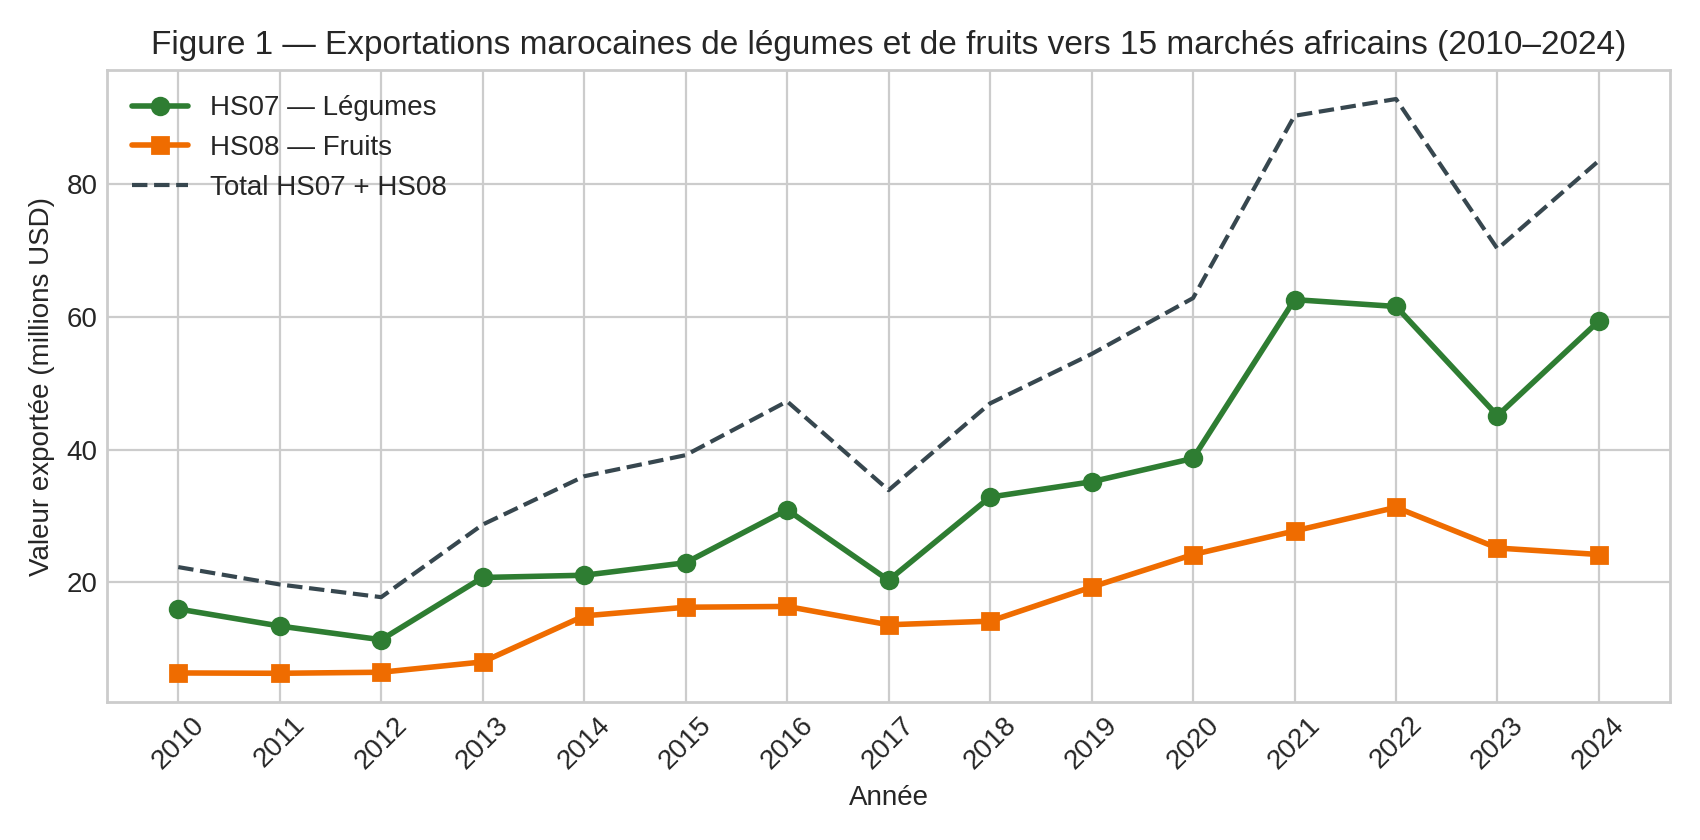
\includegraphics[width=0.88\linewidth]{figures/fig1_evolution.png}
\caption{Exportations marocaines de légumes (HS07) et de fruits (HS08) vers les quinze partenaires, par année}\label{fig:f1}
\end{figure}
Les exportations cumulées des deux chapitres vers les 15 partenaires passent de 22,28 millions USD en 2010 à 83,55 millions USD en 2024, soit un taux de croissance annuel moyen de 9,9 \%. Le maximum est atteint en 2022 (92,84 millions USD). Sur l'ensemble de la période, les légumes (HS07) représentent 66,0 \% de la valeur exportée. La trajectoire n'est pas régulière : le recul annuel le plus marqué est observé en 2017 (-28,3 \% par rapport à l'année précédente), ce qui illustre la sensibilité de ces flux aux campagnes agricoles et aux conditions d'acheminement.

\subsection{Principaux marchés}
\begin{figure}[H]\centering
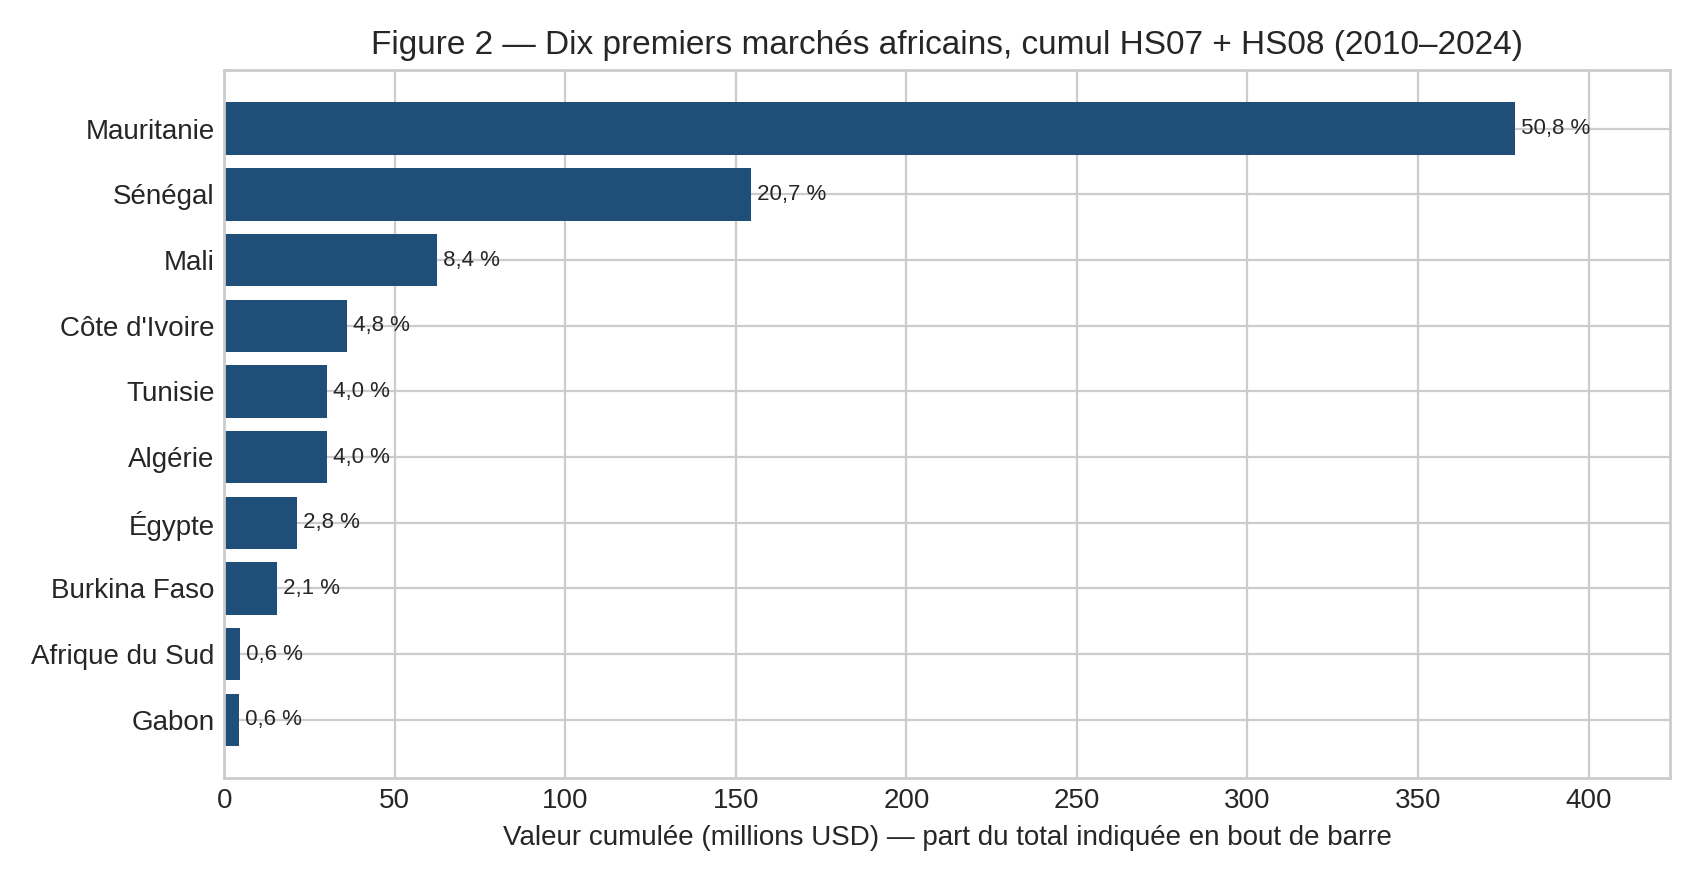
\includegraphics[width=0.88\linewidth]{figures/fig2_top_marches.png}
\caption{Dix premiers marchés africains en valeur cumulée}\label{fig:f2}
\end{figure}
Les cinq premiers marchés sont Mauritanie (378,5 M USD, 50,8 \%), Sénégal (154,4 M USD, 20,7 \%), Mali (62,5 M USD, 8,4 \%), Côte d'Ivoire (35,9 M USD, 4,8 \%) et Tunisie (30,1 M USD, 4,0 \%). Les trois premiers concentrent 79,8 \% de la valeur cumulée et les cinq premiers 88,7 \%. L'indice de Herfindahl-Hirschman calculé sur les 15 partenaires vaut 3 144, ce qui correspond à un portefeuille de marchés très concentré. Parmi les cinq premiers marchés, quatre se situent en Afrique de l'Ouest, zone desservie par la route via la Mauritanie.

\subsection{Taille du marché et croissance}
\begin{figure}[H]\centering
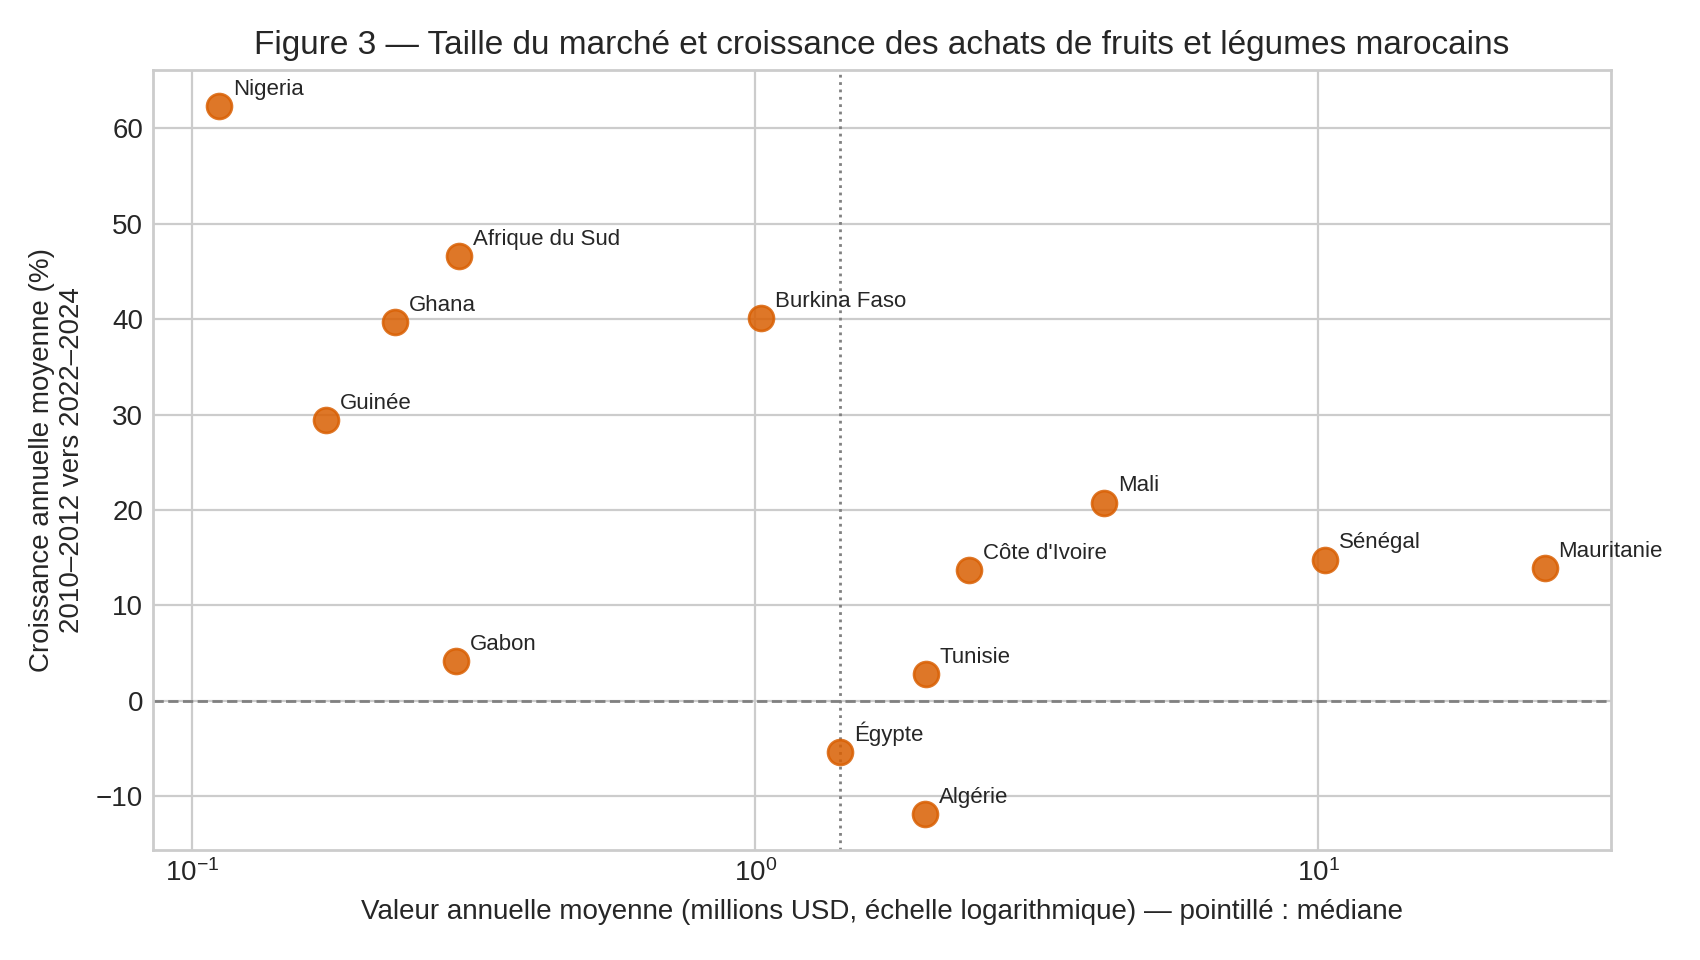
\includegraphics[width=0.88\linewidth]{figures/fig3_taille_croissance.png}
\caption{Valeur annuelle moyenne et croissance annuelle moyenne par marché}\label{fig:f3}
\end{figure}
La croissance compare la moyenne des années 2010–2012 à celle des années 2022–2024, afin de lisser les à-coups annuels. Marchés de grande taille en croissance : Mali (+20,8 \% par an), Sénégal (+14,8 \% par an), Mauritanie (+13,9 \% par an), Côte d'Ivoire (+13,7 \% par an) et Tunisie (+2,8 \% par an). Marchés de petite taille en croissance : Nigeria (+62,4 \% par an), Afrique du Sud (+46,7 \% par an), Burkina Faso (+40,1 \% par an), Ghana (+39,7 \% par an), Guinée (+29,4 \% par an) et Gabon (+4,2 \% par an). Marchés en recul : Algérie (-11,9 \% par an) et Égypte (-5,4 \% par an). Marchés sans flux en début de période et actifs en fin de période (taux non calculable, absents du graphique) : Cameroun et Kenya. Un taux élevé sur un petit marché porte sur de faibles montants : il signale un potentiel à confirmer, pas un débouché acquis.

\subsection{Légumes ou fruits selon le marché}
\begin{figure}[H]\centering
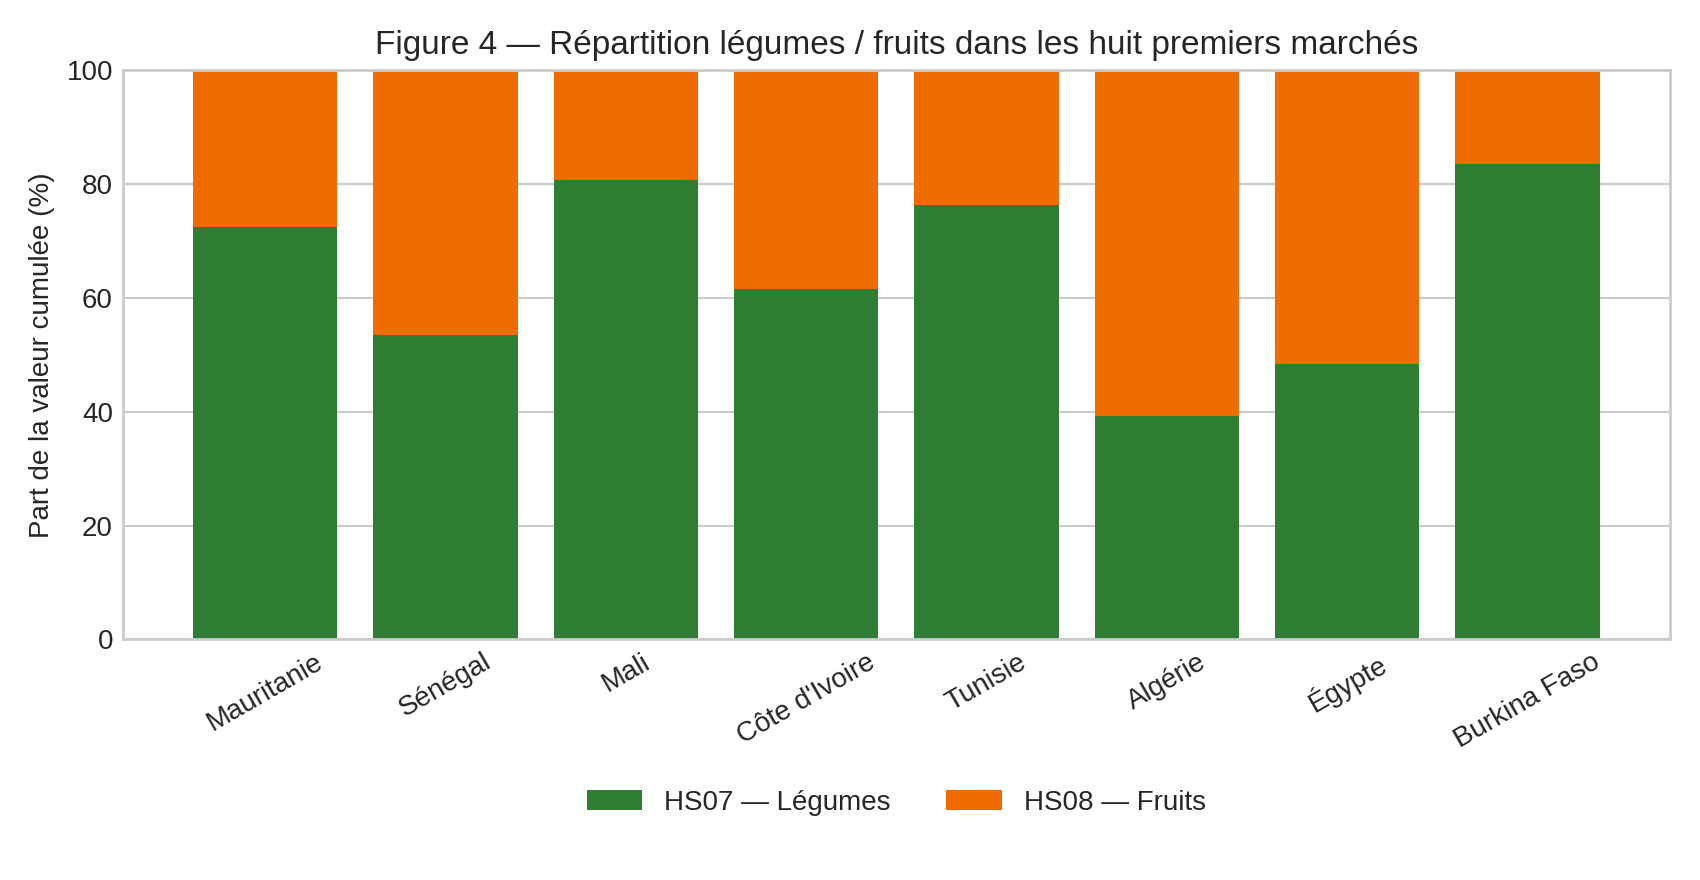
\includegraphics[width=0.85\linewidth]{figures/fig4_structure.png}
\caption{Part des chapitres HS07 et HS08 dans les huit premiers marchés}\label{fig:f4}
\end{figure}
Les légumes dominent dans Mauritanie (73 \%), Sénégal (54 \%), Mali (81 \%), Côte d'Ivoire (62 \%), Tunisie (76 \%) et Burkina Faso (83 \%). Les fruits dominent dans Algérie (61 \%) et Égypte (52 \%). Le profil de la demande diffère donc d'un marché à l'autre : l'offre à mettre en avant (légumes d'un côté, fruits de l'autre) doit être adaptée à chaque destination plutôt que définie pour l'ensemble du continent.

\subsection{Régularité des flux}
\begin{figure}[H]\centering
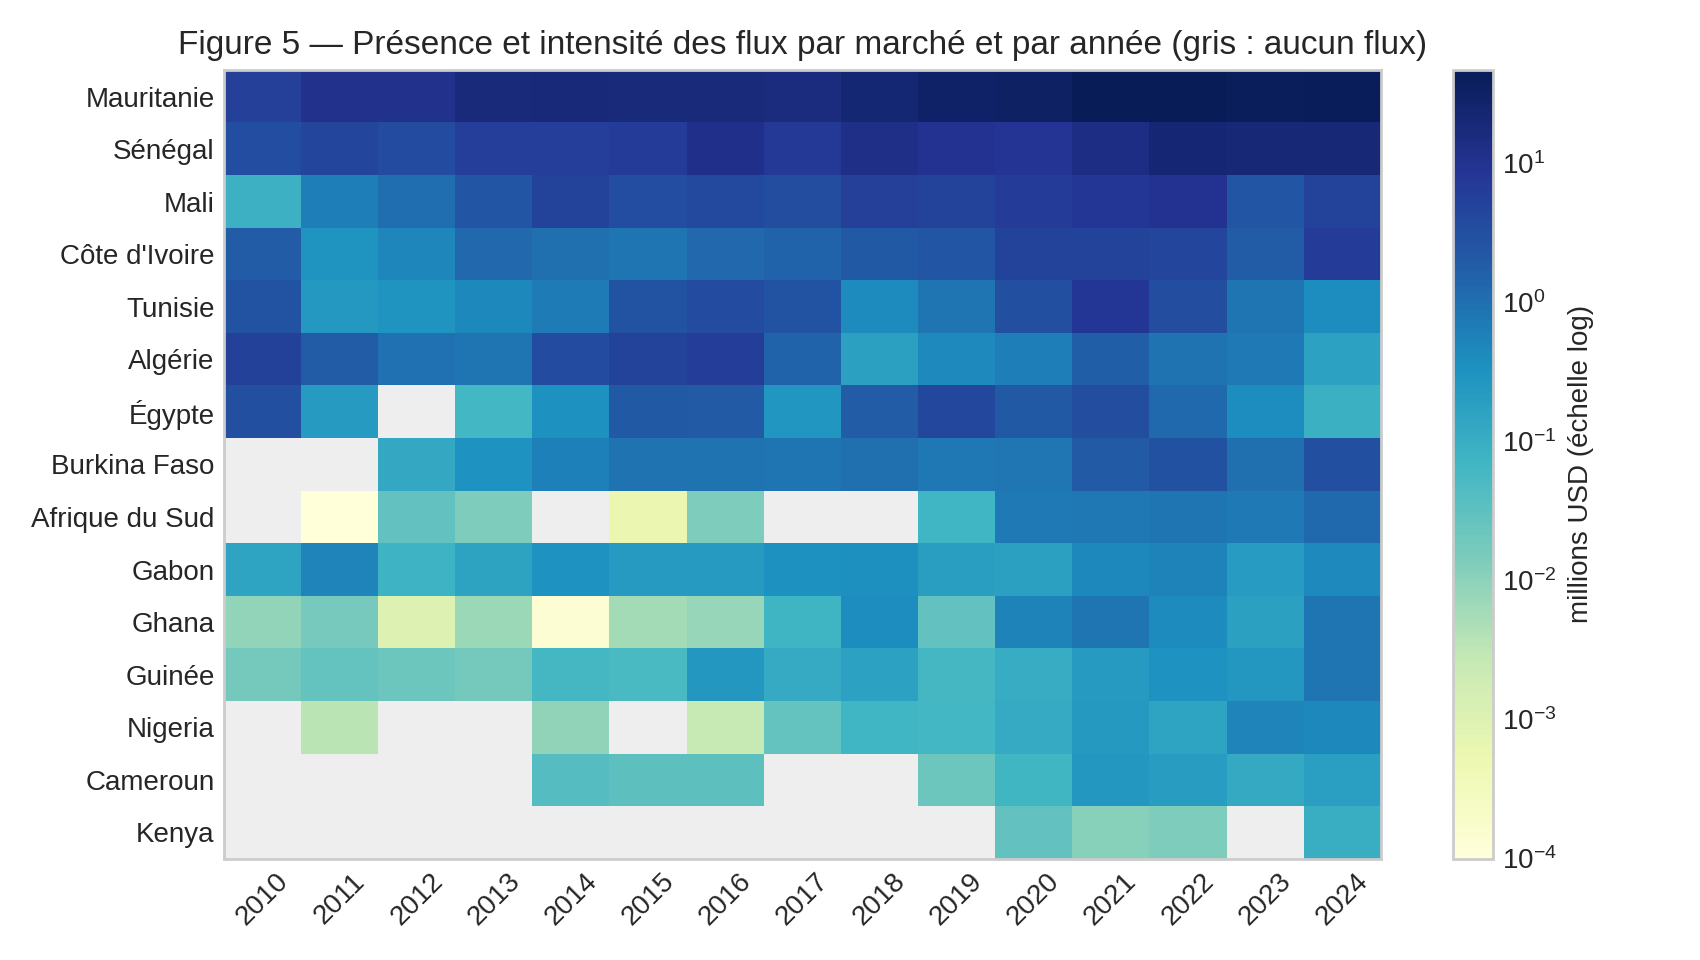
\includegraphics[width=0.88\linewidth]{figures/fig5_couverture.png}
\caption{Présence et intensité des flux par marché et par année}\label{fig:f5}
\end{figure}
Le nombre de partenaires recevant au moins un flux varie de 10 (en 2010) à 15 (en 2020) sur 15. 9 marchés sont servis chaque année sans interruption. Les flux sont intermittents vers Égypte, Burkina Faso, Afrique du Sud, Nigeria, Cameroun et Kenya. Au total, 23,1 \% des cases du panel pays × chapitre × année sont des zéros commerciaux. Cette intermittence rend les taux de croissance instables sur les petits marchés et justifie de mesurer l'erreur de prévision en valeur (millions USD) plutôt qu'en pourcentage.

\section{Méthodologie}\label{sec:method}
\subsection{Prétraitement et protocole}
La tâche est une prévision à un an : à la fin de l'année $t$, on cherche la valeur exportée vers chaque couple pays--chapitre en $t+1$. La croissance attendue se déduit de l'écart entre cette prévision et la valeur observée en $t$. Prévoir directement un taux de croissance aurait été instable, car de nombreux flux sont nuls ou très faibles.

Les variables explicatives n'utilisent que l'information disponible en $t$ : valeur de l'année $t$, des années $t-1$ et $t-2$, variation récente, moyenne sur trois ans et indicatrice du chapitre. Les retards sont calculés à l'intérieur de chaque série pays--chapitre. Les couples pays--chapitre sans aucun flux sur toute la période sont retirés. La base de modélisation compte 348 observations pour 29 séries actives.

Le découpage est strictement chronologique. Les deux dernières années disponibles ($t$ = 2022--2023, soit les cibles 2023--2024) forment le jeu de test (58 observations) et ne servent qu'à l'évaluation finale. Les années antérieures ($t$ = 2012--2021, 290 observations) servent à l'apprentissage et au réglage. Les hyperparamètres sont choisis par validation temporelle (\texttt{TimeSeriesSplit}) appliquée aux années et non aux lignes, de sorte qu'une année n'apparaît jamais à la fois en apprentissage et en validation (tableau~\ref{tab:plis}). L'imputation et la standardisation font partie des \texttt{Pipeline} scikit-learn~\cite{sklearn} et sont donc réajustées sur les seules données d'apprentissage de chaque pli.
\begin{table}[H]\centering\small
\caption{Plis de validation temporelle}\label{tab:plis}
\begin{tabular}{cllrr}\toprule
Pli & Apprentissage (années $t$) & Validation (années $t$) & $n$ apprentissage & $n$ validation \\ \midrule
1 & 2012--2015 & 2016--2017 & 116 & 58 \\
2 & 2012--2017 & 2018--2019 & 174 & 58 \\
3 & 2012--2019 & 2020--2021 & 232 & 58 \\
\bottomrule\end{tabular}
\end{table}

\subsection{Modèles}
\textbf{Référence : persistance.} La prévision est la dernière valeur observée. C'est la règle qu'appliquerait un exportateur sans modèle.

\textbf{Modèle 1 : régression Ridge.} Modèle linéaire régularisé, adapté à des variables explicatives très corrélées entre elles (valeurs retardées) et à un échantillon réduit.

\textbf{Modèle 2 : forêt aléatoire.} Moyenne d'arbres de régression construits sur des rééchantillonnages des données ; elle peut capter des effets de seuil et des interactions sans hypothèse de linéarité.

\subsection{Équations et notations}
La persistance s'écrit
\begin{equation}\label{eq:pers}
\widehat{y}_{i,k,t+1} = y_{i,k,t},
\end{equation}
où $y_{i,k,t}$ est la valeur exportée (en millions USD) vers le partenaire $i$ pour le chapitre $k$ l'année $t$, et $\widehat{y}_{i,k,t+1}$ la prévision pour l'année suivante.

La régression Ridge choisit les coefficients qui minimisent
\begin{equation}\label{eq:ridge}
\sum_{j=1}^{n}\left(y_j - \beta_0 - \mathbf{x}_j^{\top}\boldsymbol{\beta}\right)^2 + \alpha \sum_{p=1}^{P}\beta_p^2 ,
\end{equation}
où $n$ est le nombre d'observations d'apprentissage, $y_j$ la cible de l'observation $j$, $\mathbf{x}_j$ le vecteur de ses $P$ variables explicatives standardisées, $\beta_0$ la constante, $\boldsymbol{\beta} = (\beta_1,\dots,\beta_P)$ les coefficients et $\alpha \geq 0$ l'hyperparamètre qui règle l'intensité de la pénalité.

La forêt aléatoire prédit
\begin{equation}\label{eq:rf}
\widehat{y}(\mathbf{x}) = \frac{1}{B}\sum_{b=1}^{B} T_b(\mathbf{x}),
\end{equation}
où $B$ est le nombre d'arbres et $T_b(\mathbf{x})$ la prédiction de l'arbre $b$ pour le vecteur de variables $\mathbf{x}$.

Les erreurs sont mesurées par
\begin{equation}\label{eq:metriques}
\mathrm{MAE}=\frac{1}{m}\sum_{j=1}^{m}\left|y_j-\widehat{y}_j\right|,\qquad
\mathrm{RMSE}=\sqrt{\frac{1}{m}\sum_{j=1}^{m}\left(y_j-\widehat{y}_j\right)^2},\qquad
\mathrm{WAPE}=100\times\frac{\sum_{j=1}^{m}\left|y_j-\widehat{y}_j\right|}{\sum_{j=1}^{m}\left|y_j\right|},
\end{equation}
où $m$ est le nombre d'observations évaluées, $y_j$ la valeur réelle et $\widehat{y}_j$ la valeur prévue. La MAE et la RMSE s'expriment en millions USD, l'unité des échanges ; la RMSE pénalise davantage les grosses erreurs. Le WAPE rapporte l'erreur totale au total des échanges réels : contrairement au MAPE, il reste défini lorsque certains flux sont nuls.

\section{Résultats expérimentaux}\label{sec:results}
\subsection{Hyperparamètres retenus}
\begin{table}[H]\centering\small
\caption{Grilles explorées et valeurs retenues par validation temporelle (critère : MAE)}\label{tab:hyper}
\begin{tabular}{lp{7.2cm}p{4.6cm}}\toprule
Modèle & Grille explorée & Valeur retenue \\ \midrule
Ridge & $\alpha \in \{0{,}01 ; 0{,}1 ; 1 ; 10 ; 100\}$ & $\alpha$ = 0,01 \\
Forêt aléatoire & profondeur maximale $\in \{3 ; 5 ; \text{libre}\}$, taille minimale des feuilles $\in \{1 ; 3 ; 5\}$, 200 arbres & profondeur = 3, feuilles = 1 \\
\bottomrule\end{tabular}
\end{table}

\subsection{Comparaison des performances}
\begin{table}[H]\centering
\caption{Performances des trois approches (millions USD ; WAPE en \%)}\label{tab:performances}
\begin{tabular}{lrrrr}\toprule
Méthode & MAE validation & MAE test & RMSE test & WAPE test \\ \midrule
Persistance & 0,730 & 0,809 & 1,596 & 30,520 \\
Ridge & 0,767 & 1,165 & 2,400 & 43,921 \\
Forêt aléatoire & 0,966 & 0,896 & 1,560 & 33,807 \\
\bottomrule\end{tabular}
\end{table}
Sur le jeu de test, la persistance obtient une MAE de 0,809 M USD (WAPE 30,5 \%), Ridge 1,165 M USD (WAPE 43,9 \%) et la forêt aléatoire 0,896 M USD (WAPE 33,8 \%). Le modèle sélectionné sur la seule validation est « Persistance » ; le modèle le plus précis sur le test est « Persistance ». Le meilleur modèle appris (Ridge) ne fait pas mieux que la persistance sur le test (erreur supérieure de 43,9 \%) : avec des séries annuelles aussi courtes, reconduire la dernière valeur observée reste la prévision la plus fiable. Le choix du modèle se fait sur la colonne de validation ; le jeu de test n'intervient qu'ensuite, pour mesurer l'erreur attendue sur des années jamais vues.
\begin{figure}[H]\centering
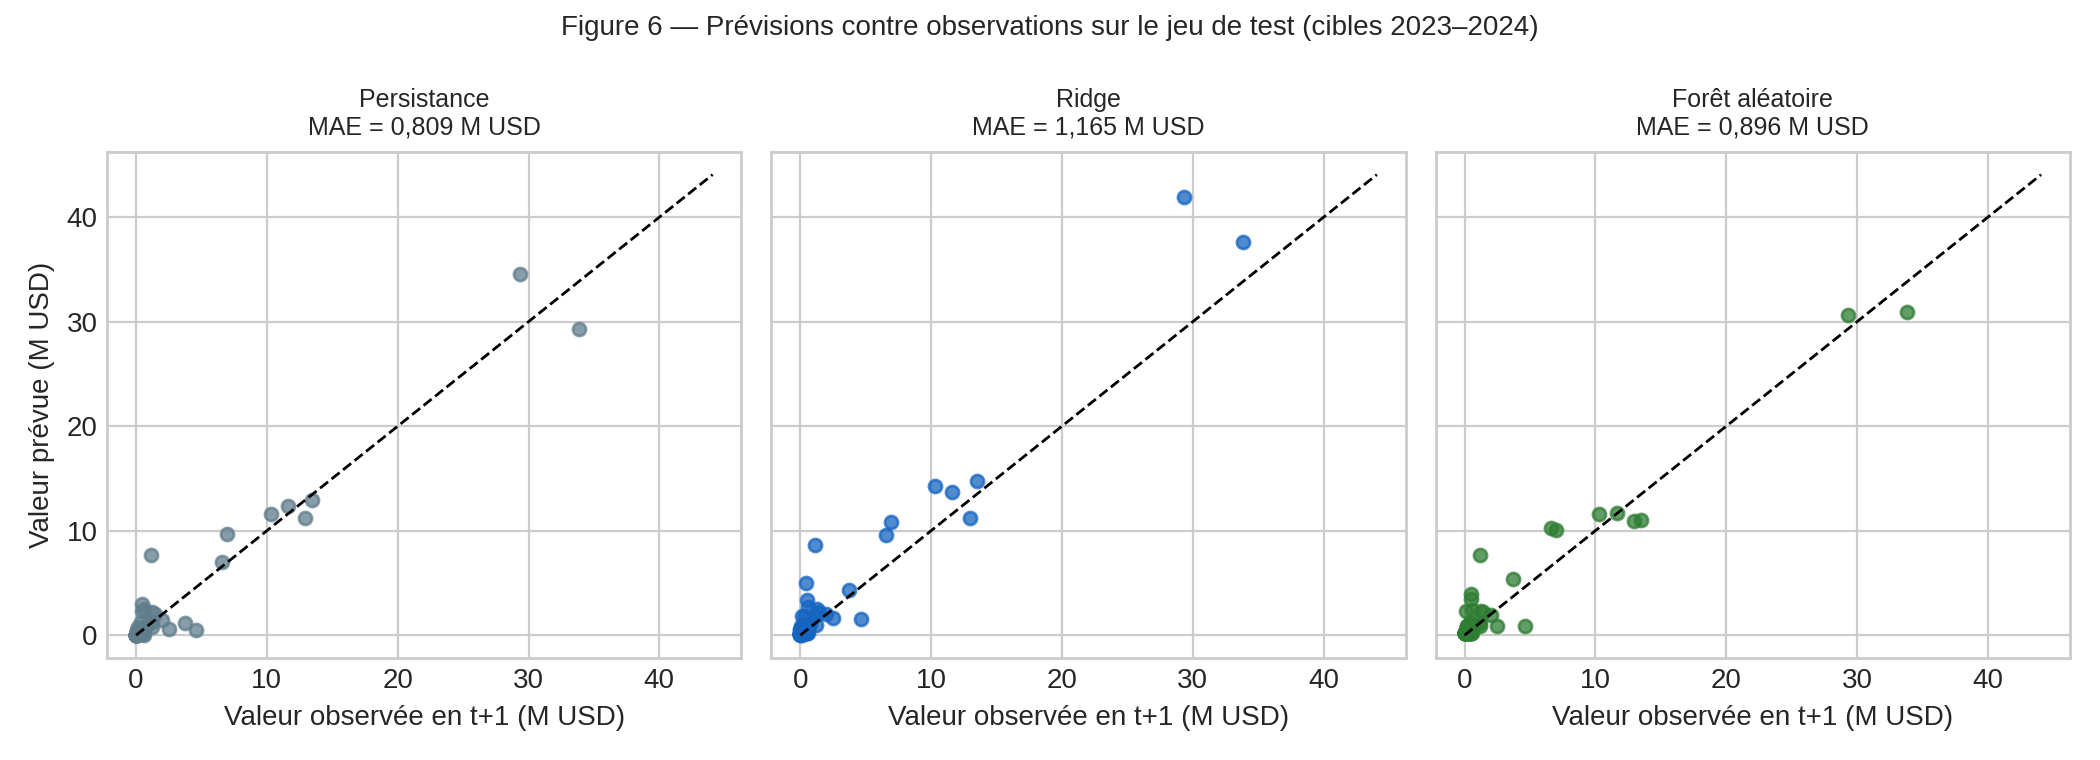
\includegraphics[width=\linewidth]{figures/fig6_prevu_observe.png}
\caption{Valeurs prévues et valeurs observées sur le jeu de test ; la diagonale correspond à une prévision parfaite}\label{fig:f6}
\end{figure}
\begin{figure}[H]\centering
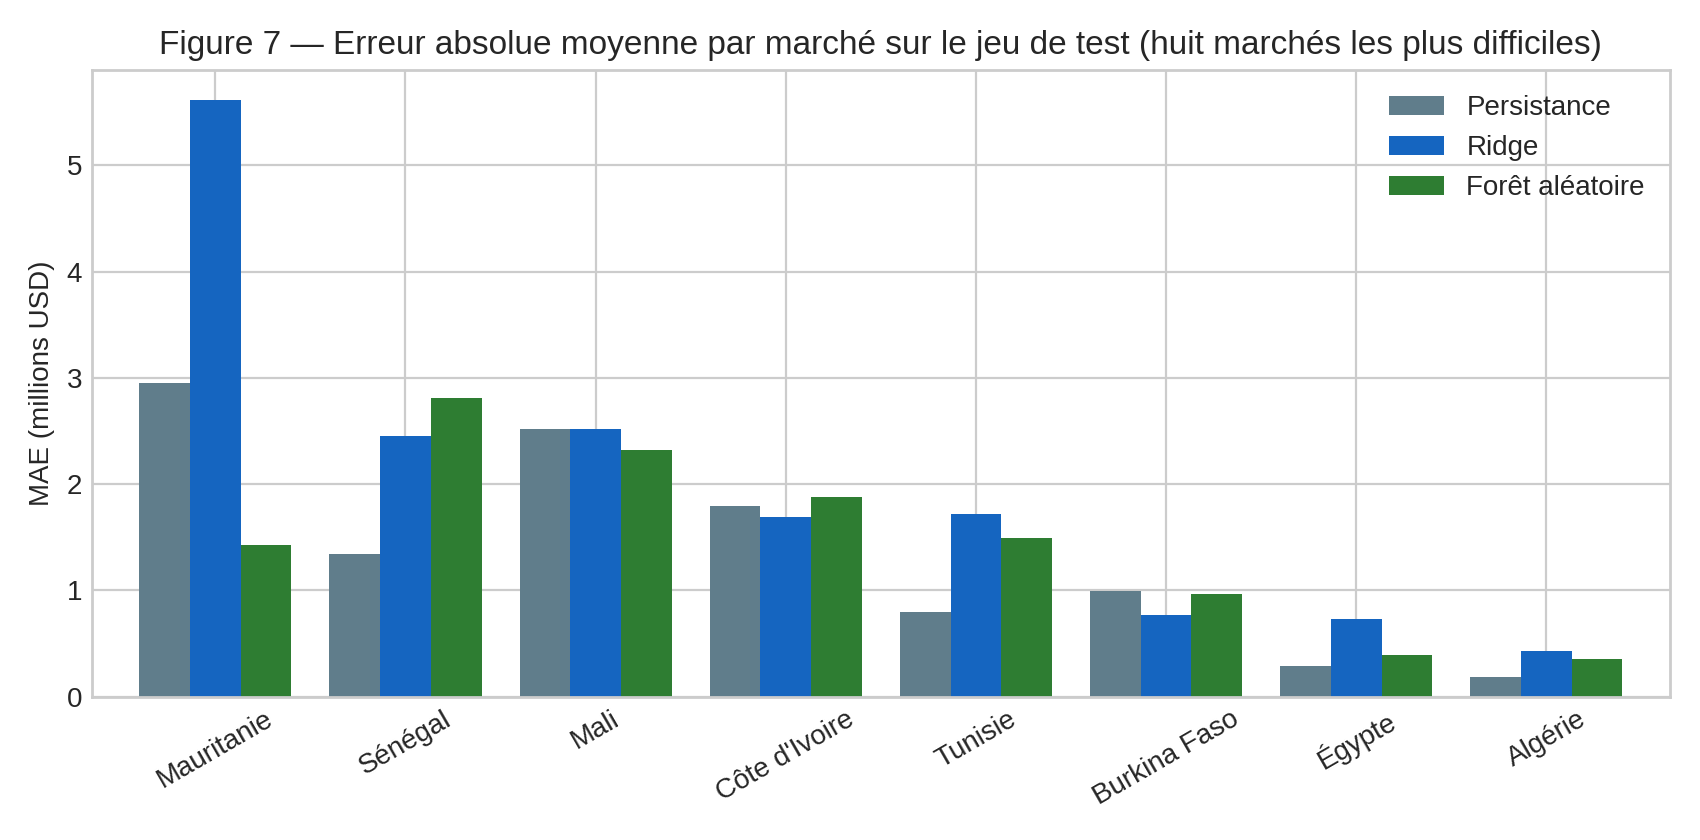
\includegraphics[width=0.85\linewidth]{figures/fig7_erreur_par_marche.png}
\caption{Erreur absolue moyenne par marché sur le jeu de test}\label{fig:f7}
\end{figure}
Les erreurs se concentrent sur Mauritanie, Sénégal et Mali : ces trois marchés représentent 62,7 \% de l'erreur absolue totale du modèle Ridge. Ce sont les marchés où les montants sont les plus élevés ou les plus irréguliers ; les petits marchés pèsent peu dans l'erreur en valeur.

\subsection{Sensibilité des conclusions}
\begin{figure}[H]\centering
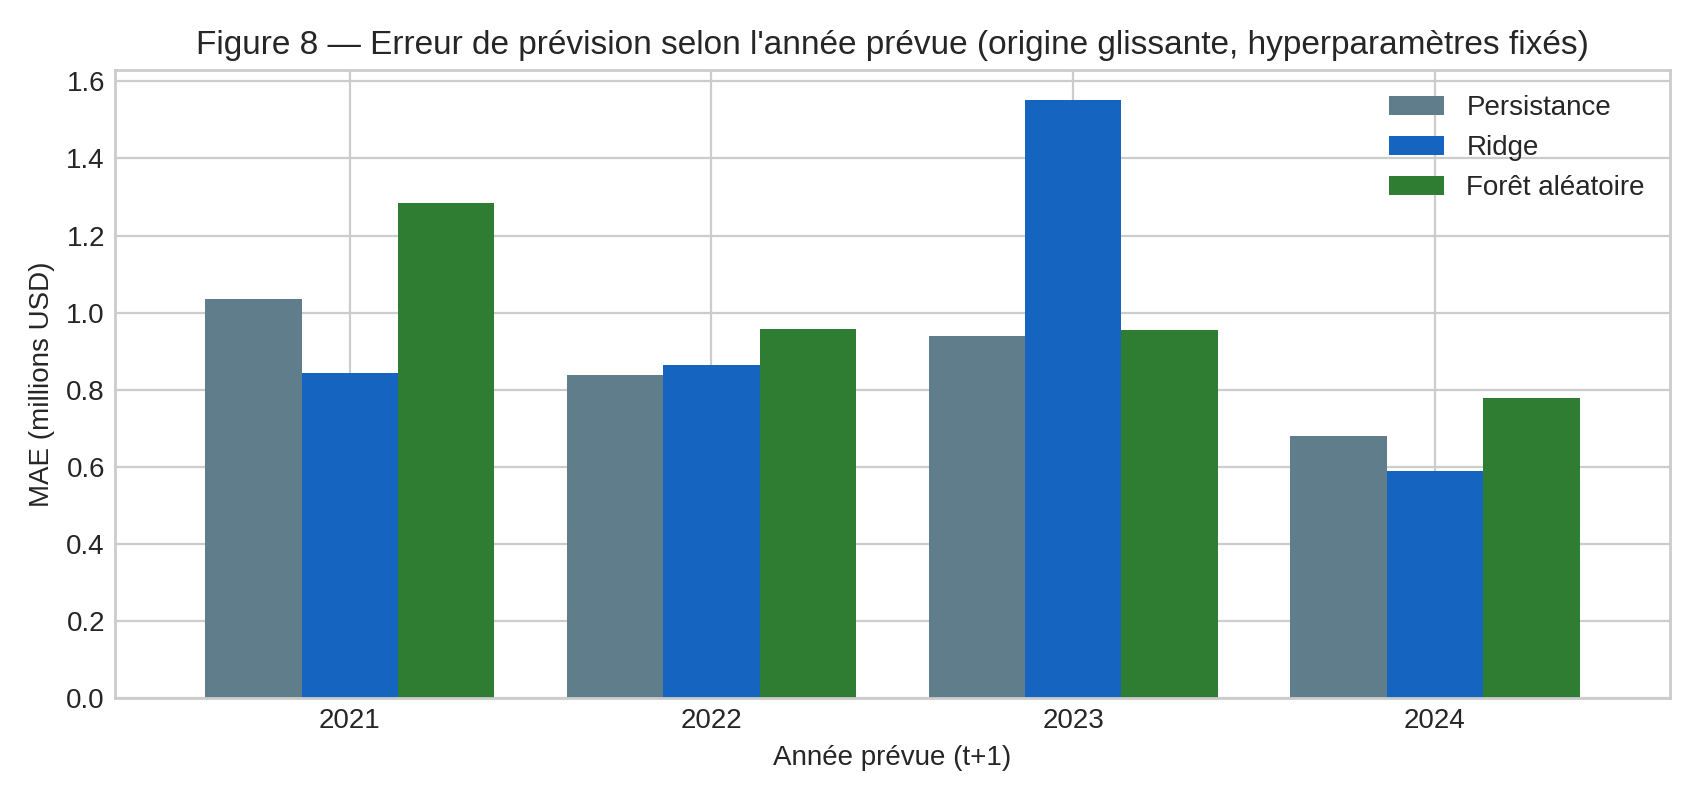
\includegraphics[width=0.85\linewidth]{figures/fig8_origine_glissante.png}
\caption{MAE selon l'année prévue : chaque modèle est réajusté sur les seules années antérieures, hyperparamètres fixés}\label{fig:f8}
\end{figure}
\begin{table}[H]\centering\small
\caption{MAE (millions USD) selon l'année prévue}\label{tab:glissant}
\begin{tabular}{crrr}\toprule
Année prévue & Persistance & Ridge & Forêt aléatoire \\ \midrule
2021 & 1,036 & 0,843 & 1,284 \\
2022 & 0,839 & 0,865 & 0,957 \\
2023 & 0,939 & 1,551 & 0,955 \\
2024 & 0,680 & 0,589 & 0,780 \\
\bottomrule\end{tabular}
\end{table}
\begin{table}[H]\centering\small
\caption{WAPE (\%) par chapitre sur le jeu de test}\label{tab:chapitre}
\begin{tabular}{lrrrr}\toprule
Chapitre & $n$ & Persistance & Ridge & Forêt aléatoire \\ \midrule
Légumes (HS07) & 28 & 33,4 & 43,9 & 34,4 \\
Fruits (HS08) & 30 & 24,4 & 44,0 & 32,6 \\
\bottomrule\end{tabular}
\end{table}
\begin{figure}[H]\centering
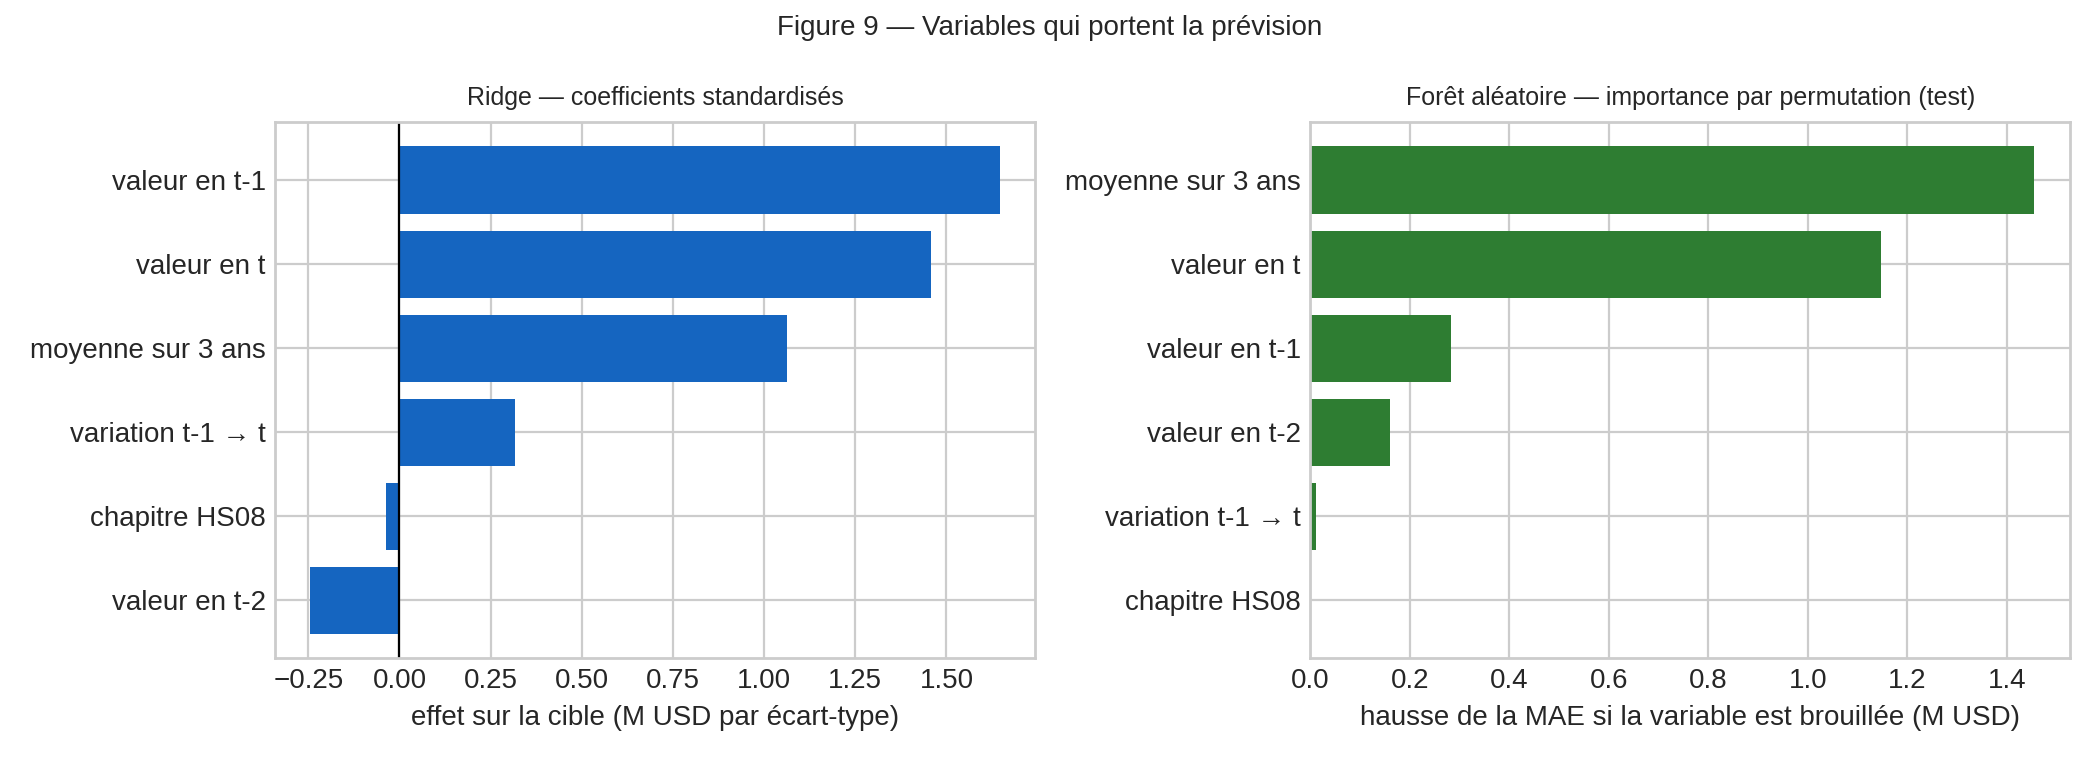
\includegraphics[width=\linewidth]{figures/fig9_variables.png}
\caption{Coefficients standardisés de Ridge et importance par permutation de la forêt aléatoire}\label{fig:f9}
\end{figure}
En rejouant la prévision pour les années 2021 à 2024, « Ridge » obtient la plus faible erreur 2 fois et « Persistance » obtient la plus faible erreur 2 fois sur 4. Le classement des modèles change donc selon l'année : aucun ne domine systématiquement, et les écarts entre eux doivent être lus avec prudence. Par chapitre, le WAPE du modèle Ridge est de 43,9 \% pour les légumes et de 44,0 \% pour les fruits : les flux de fruits sont les plus difficiles à prévoir. La variable la plus influente est « valeur en t-1 » pour Ridge et « moyenne sur 3 ans » pour la forêt aléatoire ; la corrélation entre la valeur en t et la valeur en t+1 atteint 0,95 sur l'échantillon d'entraînement. Ces importances décrivent ce que les modèles utilisent pour prévoir : elles ne démontrent aucun lien de cause à effet.

\subsection{Contrôle par le flux miroir}\label{sec:miroir}
\begin{table}[H]\centering\small
\caption{Comparaison avec le flux miroir : nombre d'années où le partenaire déclare une importation depuis le Maroc, puis cumuls en millions USD sur les couples pays--année présents dans les deux sources}\label{tab:miroir}
\begin{tabular}{lrrrr}\toprule
Pays & Années déclarées & Export Maroc (X) & Import partenaire (M) & M / X \\ \midrule
Mauritanie & 15 & 378,46 & 372,98 & 0,99 \\
Sénégal & 15 & 154,37 & 43,06 & 0,28 \\
Mali & 12 & 51,42 & 58,45 & 1,14 \\
Côte d'Ivoire & 15 & 35,94 & 36,14 & 1,01 \\
Tunisie & 15 & 30,15 & 16,01 & 0,53 \\
Algérie & 9 & 25,45 & 27,81 & 1,09 \\
Égypte & 15 & 21,23 & 19,83 & 0,93 \\
Burkina Faso & 14 & 15,33 & 4,25 & 0,28 \\
Afrique du Sud & 15 & 4,47 & 11,50 & 2,57 \\
Gabon & 14 & 3,97 & 5,04 & 1,27 \\
Ghana & 14 & 2,88 & 2,98 & 1,03 \\
Guinée & 4 & 0,39 & 0,09 & 0,22 \\
Nigeria & 13 & 1,67 & 15,27 & 9,14 \\
Cameroun & 14 & 0,77 & 0,54 & 0,70 \\
Kenya & 7 & 0,15 & 0,12 & 0,85 \\
\bottomrule\end{tabular}
\end{table}
Le tableau~\ref{tab:miroir} compare, pour chaque partenaire, les deux déclarations d'un même flux. Les partenaires ont déclaré au moins une importation de HS07 ou HS08 en provenance du Maroc pour 84,9 \% des couples pays–année possibles. Sur les 173 couples pays–année présents dans les deux sources, la corrélation entre exportations déclarées par le Maroc et importations déclarées par le partenaire est de 0,91, et les importations déclarées représentent 0,85 fois les exportations déclarées. Les deux sources ne sont pas interchangeables : l'importation est valorisée CAF (coût, assurance et fret inclus) et l'exportation FOB, les dates d'enregistrement diffèrent et certains flux transitent par un pays tiers. La couverture du flux miroir est bonne ; les déclarations marocaines sont conservées pour disposer d'un déclarant unique et d'une valorisation homogène.

\section{Discussion}\label{sec:discussion}
\subsection{Retour sur les hypothèses}
\begin{itemize}
\item \textbf{H1 (concentration)} est confirmée : les trois premiers marchés concentrent 79,8 \% de la valeur cumulée ; quatre des cinq premiers marchés se situent en Afrique de l'Ouest.
\item \textbf{H2 (persistance)} est confirmée : la corrélation entre t et t+1 vaut 0,95 et aucun modèle appris ne fait mieux que la persistance sur le test.
\item \textbf{H3 (non-linéarité)} est soutenue sur le test : la forêt aléatoire (MAE 0,896) fait mieux que Ridge (MAE 1,165).
\end{itemize}

\subsection{Lecture pour un exportateur}
Le tableau~\ref{tab:prev} applique le modèle Ridge, réajusté sur toutes les années disponibles, à la dernière année observée (2024) pour obtenir une prévision 2025 par marché.
\begin{table}[H]\centering\small
\caption{Prévision 2025 par marché (HS07 + HS08, millions USD), modèle Ridge, classée par variation décroissante}\label{tab:prev}
\begin{tabular}{lrrrr}\toprule
Pays & Valeur 2024 & Prévision 2025 & Variation & Variation (\%) \\ \midrule
Mauritanie & 44,14 & 48,53 & 4,39 & 9,96 \\
Sénégal & 20,06 & 22,16 & 2,10 & 10,49 \\
Mali & 4,91 & 6,24 & 1,33 & 27,00 \\
Tunisie & 0,40 & 1,10 & 0,70 & 174,66 \\
Égypte & 0,09 & 0,49 & 0,40 & 468,52 \\
Algérie & 0,17 & 0,52 & 0,35 & 208,46 \\
Burkina Faso & 3,06 & 3,41 & 0,35 & 11,29 \\
Gabon & 0,45 & 0,69 & 0,24 & 53,91 \\
Afrique du Sud & 1,19 & 1,42 & 0,23 & 19,22 \\
Côte d'Ivoire & 6,60 & 6,82 & 0,22 & 3,32 \\
Cameroun & 0,18 & 0,40 & 0,21 & 114,74 \\
Nigeria & 0,47 & 0,65 & 0,19 & 40,19 \\
Ghana & 0,87 & 1,04 & 0,17 & 19,54 \\
Guinée & 0,87 & 1,03 & 0,16 & 17,81 \\
Kenya & 0,09 & 0,12 & 0,03 & 29,45 \\
\bottomrule\end{tabular}
\end{table}
Consolider les marchés de grande taille en croissance (Mali, Sénégal, Mauritanie et Côte d'Ivoire), qui portent l'essentiel de la valeur. Tester à petite échelle les marchés de petite taille en progression (Nigeria, Afrique du Sud, Burkina Faso et Ghana), en gardant à l'esprit que leurs taux de croissance portent sur de faibles montants. Comprendre les causes du recul observé vers Algérie et Égypte avant d'y réinvestir. Comme aucun modèle appris ne bat la persistance sur le test, la prévision 2025 la plus prudente consiste à reconduire les valeurs de 2024 ; les priorités ci-dessus reposent sur la structure et la croissance observées, pas sur le modèle.

\subsection{Limites}
\begin{itemize}
\item \textbf{Séries courtes et annuelles.} Chaque marché ne fournit qu'une quinzaine de points. La saisonnalité des campagnes agricoles, essentielle pour des produits frais, est invisible à cette fréquence.
\item \textbf{Valeurs en dollars courants.} Une hausse de valeur peut venir des prix ou du taux de change et non des quantités ; le poids net est trop souvent absent pour le vérifier.
\item \textbf{Zéros commerciaux.} L'absence de flux et le flux non enregistré ne peuvent pas être distingués dans la source.
\item \textbf{Périmètre.} Quinze partenaires ont été sélectionnés ; les conclusions ne valent pas pour l'ensemble du continent. Le niveau du chapitre (deux chiffres) agrège des produits très différents, par exemple tomates et légumes secs.
\item \textbf{Asymétrie des déclarations.} Les exportations déclarées par le Maroc et les importations déclarées par ses partenaires ne coïncident pas (section~\ref{sec:miroir}).
\item \textbf{Absence de causalité.} Les modèles extrapolent le passé. Aucune variable externe (revenu, droits de douane, climat, coût du transport) n'est introduite : une bonne précision ne dit rien des causes de la croissance d'un marché.
\end{itemize}

\section{Conclusion et perspectives}\label{sec:conclusion}
Entre 2010 et 2024, les exportations marocaines de légumes et de fruits vers les quinze marchés étudiés sont passées de 22,28 à 83,55 millions USD. Elles sont réparties de façon inégale : Mauritanie, Sénégal et Mali concentrent 79,8~\% de la valeur cumulée. La réponse à la première partie de la question est donc donnée par les figures~\ref{fig:f2} et~\ref{fig:f3}, qui séparent les marchés de grande taille des marchés plus petits mais en progression.

Pour la seconde partie, la comparaison des trois approches sur des années jamais vues donne une MAE de 0,809 (persistance), 1,165 (Ridge) et 0,896 (forêt aléatoire) millions USD. Aucun modèle appris ne fait mieux que la persistance ; le plus proche, Ridge, a une erreur supérieure de 43,9 \%. L'historique seul permet donc une prévision d'ordre de grandeur à un an, utile pour hiérarchiser des marchés, mais pas une prévision fine marché par marché.

Trois prolongements amélioreraient ce travail : passer à des données mensuelles et à un niveau de produit plus fin (HS à quatre ou six chiffres) avec un accès authentifié à UN Comtrade ; ajouter des variables de demande et de coût (PIB et population des partenaires via l'API de la Banque mondiale~\cite{worldbank}, droits appliqués via la base de l'OMC~\cite{wto}) ; et exprimer les flux en volume pour séparer l'effet des prix.

\begin{thebibliography}{9}
\bibitem{comtrade} Nations Unies, Division de statistique, \emph{UN Comtrade API -- Documentation}. \url{https://uncomtrade.org/docs/un-comtrade-api/}. Données extraites le 19/11/2026.
\bibitem{worldbank} Banque mondiale, \emph{Indicators API -- Documentation}. \url{https://datahelpdesk.worldbank.org/knowledgebase/articles/889392}.
\bibitem{wto} Organisation mondiale du commerce, \emph{Tariff and Trade Data}. \url{https://data.wto.org/en/dataset/wto_ttd}.
\bibitem{sklearn} F. Pedregosa et al., \emph{Scikit-learn: Machine Learning in Python}, Journal of Machine Learning Research, vol. 12, p. 2825--2830, 2011.
\bibitem{agri} Royaume du Maroc, Ministère de l'Agriculture, \emph{Stratégies Plan Maroc Vert et Génération Green 2020--2030}. \url{https://www.agriculture.gov.ma}.
\bibitem{zlecaf} Secrétariat de la ZLECAf, \emph{Zone de libre-échange continentale africaine}. \url{https://au-afcfta.org}.
\end{thebibliography}

\appendix
\section{Annexe : reproductibilité}
\sloppy
\begin{itemize}
\item \textbf{Environnement.} Python 3.13.18, numpy 2.4.6, pandas 2.2.3, scikit-learn 1.6.1, matplotlib 3.10.0, requests 2.32.4. Graine aléatoire fixée à 42.
\item \textbf{Exécution.} Le notebook s'exécute de bout en bout avec \emph{Exécution > Tout exécuter} sur Google Colab. Les données brutes reçues de l'API sont enregistrées dans \texttt{data/} ; si ces fichiers sont présents, le notebook les relit au lieu de rappeler l'API, ce qui garantit des résultats identiques.
\item \textbf{Fichiers produits.} \texttt{figures/} (neuf figures), \texttt{data/comtrade\_maroc\_exports\_brut.csv}, \texttt{data/panel\_nettoye.csv}, \texttt{data/comparaison\_modeles.csv}, \texttt{data/journal\_requetes.csv}, \texttt{data/reproductibilite.json}.
\item \textbf{Journal du binôme.} Nom Prénom 1 : extraction API et nettoyage, figures 1 à 3, modèle Ridge, sections 1 à 3 du rapport. Nom Prénom 2 : dictionnaire des variables, figures 4 et 5, forêt aléatoire et validation, sections 4 à 7 du rapport, support de soutenance.
\item \textbf{Déclaration d'usage de l'IA.} Un assistant d'intelligence artificielle générative (Claude, Anthropic) a été utilisé pour concevoir le code Python, le gabarit LaTeX et pour aider à la rédaction. Toutes les données proviennent de l'API UN Comtrade et tous les chiffres du rapport sont calculés par le notebook ; aucun résultat n'a été produit par l'assistant. Le binôme a exécuté le notebook, contrôlé les résultats et relu l'ensemble du rapport.
\end{itemize}
\end{document}
